\documentclass{beamer}
\usetheme{Singapore}
\usepackage{changepage}

%\usepackage{pstricks,pst-node,pst-tree}
\usepackage{amssymb,latexsym}
\usepackage{tikz}
\usepackage{graphicx}
\usepackage{fancyvrb}
\usepackage{hyperref}
\usepackage{fancybox}
\usepackage[listings]{tcolorbox}

\definecolor{codegreen}{rgb}{0,0.6,0}
\definecolor{codegray}{rgb}{0.5,0.5,0.5}
\definecolor{codepurple}{rgb}{0.58,0,0.82}
\definecolor{backcolour}{rgb}{0.95,0.95,0.92}

\lstdefinestyle{mystyle}{
    language=Python,
    backgroundcolor=\color{backcolour},   
    commentstyle=\color{codegreen},
    keywordstyle=\color{magenta},
    numberstyle=\tiny\color{codegray},
    stringstyle=\color{codepurple},
    basicstyle=\ttfamily\footnotesize,
    breakatwhitespace=false,         
    breaklines=true,                 
    captionpos=b,                    
    keepspaces=true,                 
    numbers=left,                    
    numbersep=5pt,                  
    showspaces=false,                
    showstringspaces=false,
    showtabs=false,                  
    tabsize=2,
    escapechar=|,
    frame=single
}

\lstset{style=mystyle}


\newcommand{\bi}{\begin{itemize}}
\newcommand{\li}{\item}
\newcommand{\ei}{\end{itemize}}
\newcommand{\Show}[1]{
\begin{center}
\shadowbox{\begin{minipage}{0.8\textwidth}
          #1
          \end{minipage}}
\end{center}
}
\newcommand{\arrow}{\ensuremath{\rightarrow}}

\newcommand{\uparr}{\ensuremath{\uparrow}}


\newcommand{\fig}[2]{\centerline{\includegraphics[width=#1\textwidth]{#2}}}

\newcommand{\bfr}[1]{\begin{frame}[fragile]\frametitle{{ #1 }}}
\newcommand{\efr}{\end{frame}}

\newcommand{\cola}{\begin{columns}\begin{column}{0.5\textwidth}}
\newcommand{\colb}{\end{column}\begin{column}{0.5\textwidth}}
\newcommand{\colc}{\end{column}\end{columns}}


\title{Think Python 2e, Chapter 16 Notes}
\author{Classes and Functions}

\begin{document}

\begin{frame}
\maketitle
\end{frame}


\bfr{A new data type:  {\tt Time}}
\begin{lstlisting}
class Time:
    """Represents the time of day.
       
    attributes: hour, minute, second
    """
\end{lstlisting}
\begin{lstlisting}
>>> time = Time()
>>> time.hour = 11
>>> time.minute = 59
>>> time.second = 30
\end{lstlisting}
Object diagram:
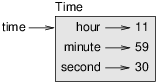
\includegraphics{statediagram16-01}

\end{frame}



\bfr{A function of time}
\begin{lstlisting}
def print_time(t):
    print('%d:%.2d:%.2d' 
            % (t.hour,t.minute,t.second))
\end{lstlisting}
\begin{lstlisting}
>>> print_time(time)
11:59:30
\end{lstlisting}
\end{frame}

\bfr{Prototype of {\tt add\_time}}
\begin{lstlisting}
def add_time(t1, t2):
    sum = Time()
    sum.hour = t1.hour + t2.hour
    sum.minute = t1.minute + t2.minute
    sum.second = t1.second + t2.second
    return sum
\end{lstlisting}
This is called a {\bf pure function} because:
\bi
\li it does not modify its arguments
\li it has no effect, like printing or reading
\li it {\bf only} returns a value
\ei
It is like a mathematical function.
\end{frame}


\bfr{Figure out when the movie ends}
\begin{lstlisting}
>>> start = Time()
>>> start.hour = 9
>>> start.minute = 45
>>> start.second =  0

>>> duration = Time()
>>> duration.hour = 1
>>> duration.minute = 35
>>> duration.second = 0

>>> done = add_time(start, duration)
>>> print_time(done)
10:80:00
\end{lstlisting}

Disappointing.


\end{frame}


\bfr{Figure out when the movie ends, improved}
\begin{lstlisting}
def add_time(t1, t2):
    sum = Time()
    sum.hour = t1.hour + t2.hour
    sum.minute = t1.minute + t2.minute
    sum.second = t1.second + t2.second

    if sum.second >= 60:
        sum.second -= 60
        sum.minute += 1

    if sum.minute >= 60:
        sum.minute -= 60
        sum.hour += 1

    return sum
\end{lstlisting}

Still not perfect.  We'll improve it later.


\end{frame}

\bfr{Modifiers}

\bi
\li Functions that have side effects are not pure functions.
\li They are called {\bf modifiers}.
\ei
\begin{lstlisting}
def increment(time, seconds):
    time.second += seconds

    if time.second >= 60:
        time.second -= 60
        time.minute += 1

    if time.minute >= 60:
        time.minute -= 60
        time.hour += 1
\end{lstlisting}

Does this really work?  What's wrong?  How would you fix it?



\end{frame}

\bfr{Pure Functions {\em vs.} Modifiers}
\bi
\li
Anything that can be done with modifiers can be done with pure functions.
\li
Programming with pure functions is called {\bf functional programming style}.
\li
Some programming languages do not allow modifiers.
\li
There is evidence that pure functions are faster to develop and less error-prone.
\li
Functional programs are occasionally less efficient due to copying.
\ei


\end{frame}

\bfr{Prototyping {\em vs.} Planning}
\bi
\li
The development we've seen in this chapter is called
{\bf prototype and patch}.
\li
Begin with a simple prototype, test it, patch it, repeat.
\li
Incremental correction can generate code that is 
unnecessarily complex and unreliable.
\li It's hard to know when you've found all the errors.
\ei
\end{frame}

\bfr{Planned development}
\bi
\li 
An alternative to prototype and patch is {\bf designed development}.
\li
Here we use a high-level understanding of the problem to restructure
the code from the beginning.
\li
As an example, the \lstinline{Time} class is really just a single
integer in base 60.
\li
The seconds are the ones, the minutes are the sixties, and the 
hours are the sixty-squareds, or thirty-six hundreds.
\li
Since time is just an integer, we can just use integer addition
to add times.
\li We just have to convert the times to integers, add them,
and convert them back.
\ei
\end{frame}

\bfr{Convert times to and from integers}
\begin{lstlisting}
def time_to_int(time):
    minutes = time.hour * 60 + time.minute
    seconds = minutes * 60 + time.second
    return seconds
\end{lstlisting}
\begin{lstlisting}
def int_to_time(seconds):
    time = Time()
    minutes, time.second = divmod(seconds, 60)
    time.hour, time.minute = divmod(minutes, 60)
    return time
\end{lstlisting}
\end{frame}

\bfr{New approach makes things MUCH easier}
\begin{lstlisting}
def add_time(t1, t2):
    seconds = time_to_int(t1) + time_to_int(t2)
    return int_to_time(seconds)
\end{lstlisting}

\end{frame}

\bfr{New approach makes things MUCH easier}
\bi
\li This version is much shorter than the original.
\li This version is correct.
\li It is easy to see it must be correct.
\li We had to see the problem abstractly.
\li We had to do more work at the start:
\bi \li write the to and from conversion functions \ei
\li It makes it easier to add more features, {\em e.g.} subtraction.
\li Sometimes making a problem harder makes it easier.
\ei
\end{frame}

\bfr{Debugging}
\bi
\li
An {\bf invariant} is something that should always be true.
\ei
\begin{lstlisting}
def valid_time(time):
    if time.hour<0 or time.minute<0 or time.second<0:
        return False
    if time.minute >= 60 or time.second >= 60:
        return False
    return True
\end{lstlisting}
\end{frame}
\bfr{Debugging}
We can use this in every function of time:
\begin{lstlisting}
def add_time(t1, t2):
    if not valid_time(t1) or not valid_time(t2):
        raise ValueError('invalid Time object')
    seconds = time_to_int(t1) + time_to_int(t2)
    return int_to_time(seconds)
\end{lstlisting}
\lstinline{assert} raises an exception when its condition is false:
\begin{lstlisting}
def add_time(t1, t2):
    assert valid_time(t1) and valid_time(t2)
    seconds = time_to_int(t1) + time_to_int(t2)
    return int_to_time(seconds)
\end{lstlisting}
Using \lstinline{assert} helps distinguish normal code from
error-checking.


\end{frame}
\bfr{Vocabulary}
\begin{description}
\li[prototype and patch:]
A development plan that involves writing a rough draft of a program, testing, and correcting errors as they are found.
\li[designed development:]
A development plan that involves high-level insight into the problem and more planning than incremental development or prototype development.
\end{description}
\end{frame}
\bfr{Vocabulary}
\begin{description}
\li[pure function:]
A function that does not modify any of the objects it receives as arguments. Most pure functions are fruitful.
\li[modifier:]
A function that changes one or more of the objects it receives as arguments. Most modifiers are void; that is, they return None.
\li[functional programming style:]
A style of program design in which the majority of functions are pure.
\end{description}
\end{frame}
\bfr{Vocabulary}
\begin{description}
\li[invariant:]
A condition that should always be true during the execution of a program.
\li[assert statement:]
A statement that checks a condition and raises an exception if it fails.
\end{description}

\end{frame}

\end{document}
